\documentclass[main.tex]{subfiles}

\begin{document}

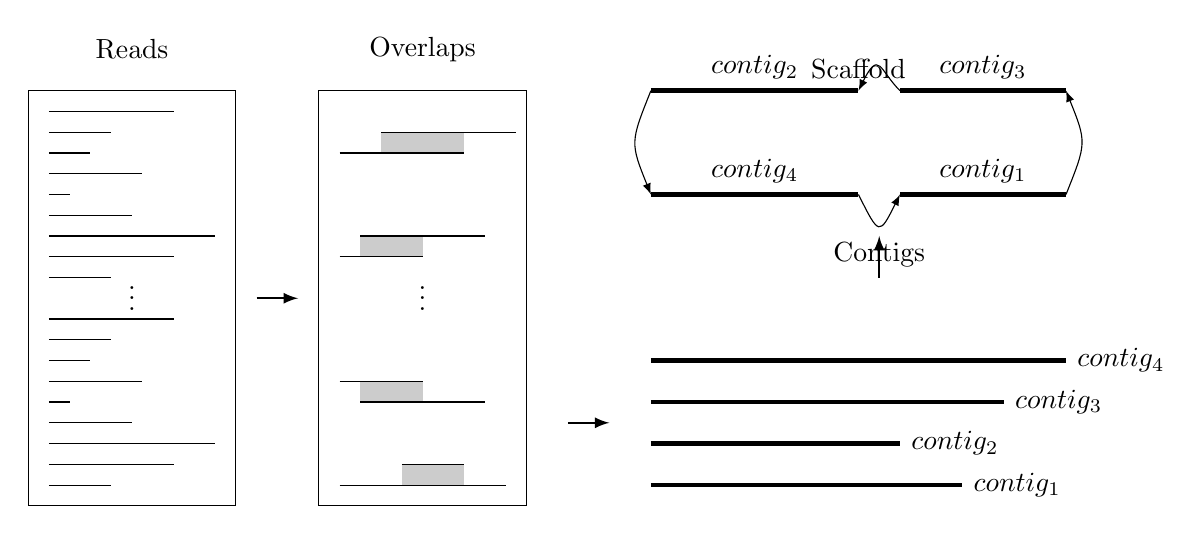
\begin{tikzpicture}[x=0.75pt,y=0.75pt]

\draw [black] (0, 0) -- (100, 0) -- (100, 200) -- (0, 200) -- cycle;
\draw (50, 220) node {Reads};

\draw [black] (10, 10) -- (40, 10);
\draw [black] (10, 20) -- (70, 20);
\draw [black] (10, 30) -- (90, 30);
\draw [black] (10, 40) -- (50, 40);
\draw [black] (10, 50) -- (20, 50);
\draw [black] (10, 60) -- (55, 60);
\draw [black] (10, 70) -- (30, 70);
\draw [black] (10, 80) -- (40, 80);
\draw [black] (10, 90) -- (70, 90);

\draw (50, 95) node {.};
\draw (50, 100) node {.};
\draw (50, 105) node {.};

\draw [black] (10, 110) -- (40, 110);
\draw [black] (10, 120) -- (70, 120);
\draw [black] (10, 130) -- (90, 130);
\draw [black] (10, 140) -- (50, 140);
\draw [black] (10, 150) -- (20, 150);
\draw [black] (10, 160) -- (55, 160);
\draw [black] (10, 170) -- (30, 170);
\draw [black] (10, 180) -- (40, 180);
\draw [black] (10, 190) -- (70, 190);

\draw [fill opacity=1, ->, >=latex,thick,black] (110, 100) -- (130, 100);

\draw [black] (140, 0) -- (240, 0) -- (240, 200) -- (140, 200) -- cycle;
\draw (190, 220) node {Overlaps};


\fill [black!20] (180, 10) rectangle (210, 20);
\draw [black] (150, 10) -- (230, 10);
\draw [black] (180, 20) -- (210, 20);

\fill [black!20] (160, 50) rectangle (190, 60);
\draw [black] (150, 60) -- (190, 60);
\draw [black] (160, 50) -- (220, 50);

\draw (190, 95) node {.};
\draw (190, 100) node {.};
\draw (190, 105) node {.};

\fill [black!20] (160, 120) rectangle (190, 130);
\draw [black] (150, 120) -- (190, 120);
\draw [black] (160, 130) -- (220, 130);

\fill [black!20] (170, 170) rectangle (210, 180);
\draw [black] (150, 170) -- (210, 170);
\draw [black] (170, 180) -- (235, 180);

\draw [fill opacity=1, ->, >=latex,thick,black] (260, 40) -- (280, 40);

\draw [black, ultra thick] (300, 10) -- (450, 10) node[right] {$contig_1$};
\draw [black, ultra thick] (300, 30) -- (420, 30) node[right] {$contig_2$};
\draw [black, ultra thick] (300, 50) -- (470, 50) node[right] {$contig_3$};
\draw [black, ultra thick] (300, 70) -- (500, 70) node[right] {$contig_4$};

\draw [fill opacity=1, ->, >=latex,thick,black] (410, 110) -- (410, 130) node[at start, above] {Contigs};

\draw [black, ultra thick] (300, 150) -- (400, 150) node[midway, above] {$contig_4$};
\draw [black, ultra thick] (420, 150) -- (500, 150) node[midway, above] {$contig_1$};
\draw [black, ultra thick] (420, 200) -- (500, 200) node[midway, above] {$contig_3$};
\draw [black, ultra thick] (300, 200) -- (400, 200) node[midway, above] {$contig_2$};

\draw [fill opacity=1, ->, >=latex, black] (400, 150)  .. controls (410, 130) and (410, 130) .. (420, 150);
\draw [fill opacity=1, ->, >=latex, black] (500, 150)  .. controls (510, 175) and (510, 175) .. (500, 200);
\draw [fill opacity=1, ->, >=latex, black] (420, 200)  .. controls (410, 210) and (410, 220) .. (400, 200);
\draw [fill opacity=1, ->, >=latex, black] (300, 200)  .. controls (290, 175) and (290, 175) .. (300, 150);

\draw (400, 220) node[below] {Scaffold};

\end{tikzpicture}

\end{document}